\documentclass[11pt]{article}

\usepackage[margin=1in]{geometry}
\usepackage[T1]{fontenc}
\usepackage[utf8]{inputenc}
\usepackage{lmodern}
\usepackage{amsmath,amssymb}
\usepackage{booktabs}
\usepackage{graphicx}
\usepackage{subcaption}
\usepackage{hyperref}

\hypersetup{colorlinks=true,linkcolor=blue,urlcolor=blue,citecolor=blue}

\title{Supplementary Materials:\\Reaction-Boundary Volatility Surface Simulations}
\author{}
\date{}

\begin{document}
\maketitle

\section{Short Background}

This supplementary note describes simulation figures generated from the
reaction-boundary volatility closure. The aim is to illustrate how structural
order-book quantities can shape a projected local-volatility surface.

\section{Reaction-Boundary Volatility Closure}

The starting point is the operational variance closure
\begin{equation}
 a_u^{(\Delta)}(S,u)
 \simeq
 \left[
 \frac{\mathcal A_{\mathrm{eff}}(S,u)}
      {\mathcal L(S,u)^2}
 \right]
 \Delta^{-\gamma(S,u)}
 \mathcal F_{\gamma(S,u)}\!\left(\nu(S,u)\Delta\right).
\end{equation}
Under a deterministic activity clock, the projected local variance is
\begin{equation}
 \sigma_{\mathrm{loc}}^2(S,t)
 =
 \alpha(t)\Xi(S,U(t);\Delta).
\end{equation}

\section{Response-Regime Approximations}

The two response regimes used in the simulations are
\begin{equation}
 \mathcal F_\gamma(z)
 \sim
 \frac{\tan(\pi\gamma/2)}{2(1-\gamma)},
 \qquad z\ll1,
\end{equation}
and
\begin{equation}
 \mathcal F_\gamma(z)
 \sim
 K_\gamma^{(0)}z^{\gamma-1},
 \qquad z\gg1,
\end{equation}
where
\begin{equation}
 K_\gamma^{(0)}
 =
 \frac{
 \Gamma(1-\gamma)\sin(\pi\gamma/2)
 \Gamma(\gamma/2)\Gamma((1-\gamma)/2)
 }{2\pi^{3/2}}.
\end{equation}

\section{Structural Simulation Profiles}

The simulations use log-moneyness
\[
 m=\ln(x/x_0)
\]
as the state coordinate. Three structural profiles are considered:
\begin{enumerate}
 \item liquidity-only;
 \item resilience-response-only;
 \item combined structural.
\end{enumerate}

\section{Numerical Implementation}

The projected variance surface is evaluated on a two-dimensional grid in
log-moneyness \(m\) and maturity \(T\). The plotted quantity is projected
local volatility,
\[
 \sigma_{\mathrm{loc}}(m,T)
 =
 \sqrt{\sigma_{\mathrm{loc}}^2(m,T)}.
\]

\section{Parameter Choices}

% Include or paste the standalone parameter-range and response-regime tables here.

\section{Simulated Surfaces}

\subsection{Liquidity-Only Profile}

% Include low-z and high-z liquidity-only surface/contour pairs here.

\subsection{Resilience-Response-Only Profile}

% Include low-z and high-z resilience-response-only surface/contour pairs here.

\subsection{Combined Structural Profile}

\begin{figure}[ht]
 \centering
 \begin{subfigure}{0.48\linewidth}
  \centering
  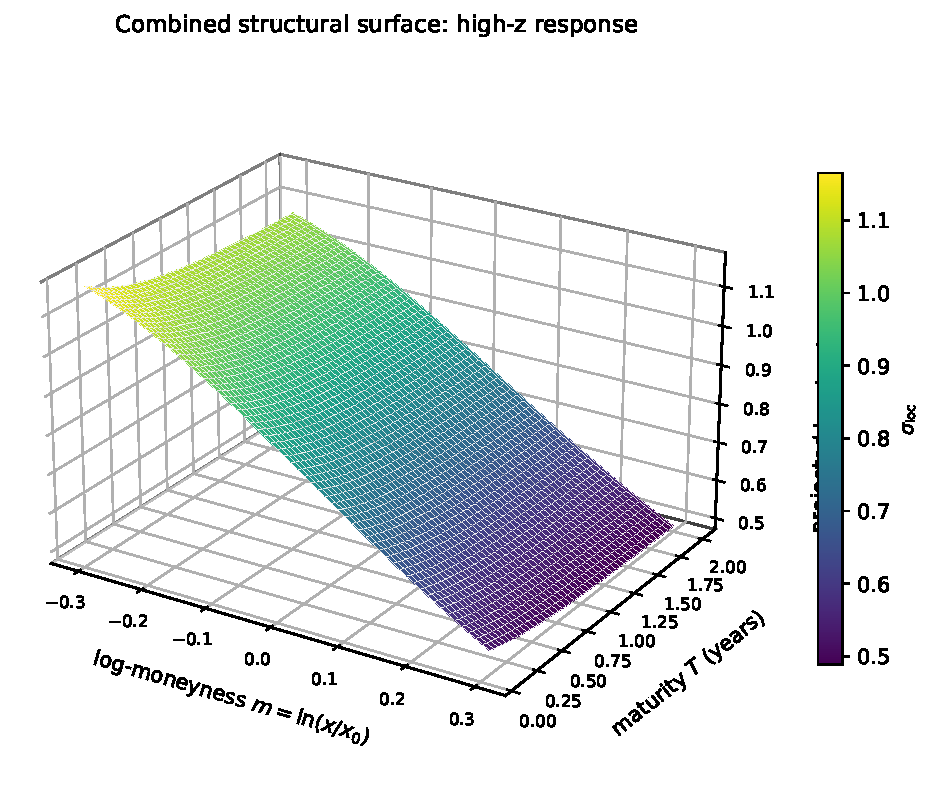
\includegraphics[width=\linewidth]{figures/mpl-surface3d-combined-structural-high-z-v3.pdf}
  \caption{Boxed surface view.}
 \end{subfigure}
 \hfill
 \begin{subfigure}{0.48\linewidth}
  \centering
  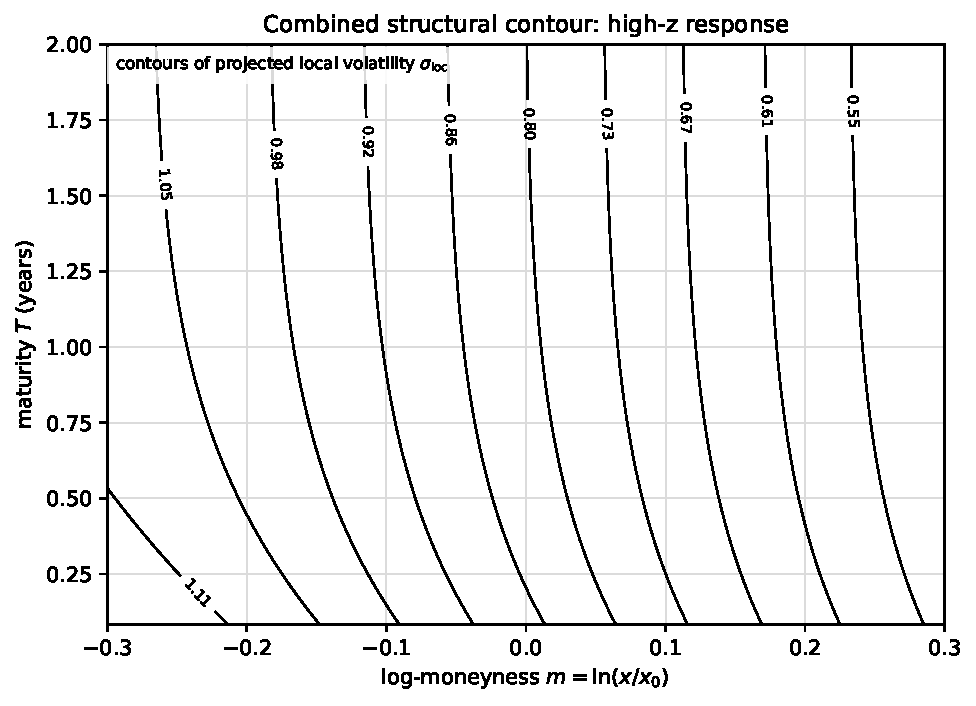
\includegraphics[width=\linewidth]{figures/mpl-contour-lines-combined-structural-high-z-v3.pdf}
  \caption{Black contour-line projection.}
 \end{subfigure}
 \caption{Projected local-volatility surface for the combined structural profile in the high-\(z\) response regime. The state coordinate is log-moneyness \(m=\ln(x/x_0)\), and \(T\) denotes maturity in years. The figure illustrates a structural simulation of the reaction-boundary closure, not an empirical calibration.}
\end{figure}

\section{Robustness Checks}

The diagnostic checks verify positivity, finite values, expected monotonicity,
and grid robustness for the simulated surfaces.

\section{Limitations And Interpretation}

The simulated surfaces are mechanism illustrations. The profiles are
structural modelling choices and should not be read as calibrated estimates
of liquidity, resilience, signed-flow intensity, or activity.

\end{document}

